% --------------------------------------------------------------
% This is all preamble stuff that you don't have to worry about.
% Head down to where it says "Start here"
% --------------------------------------------------------------
\documentclass[12pt]{article}
 
\usepackage[margin=1in]{geometry} 
\usepackage{amsmath,amsthm,amssymb}
\usepackage{actuarialsymbol}
\usepackage{graphicx}
\graphicspath{ {./images/ } }
 
\newcommand{\N}{\mathbb{N}}
\newcommand{\Z}{\mathbb{Z}}
 
\newenvironment{theorem}[2][Theorem]{\begin{trivlist}
\item[\hskip \labelsep {\bfseries #1}\hskip \labelsep {\bfseries #2.}]}{\end{trivlist}}
\newenvironment{lemma}[2][Lemma]{\begin{trivlist}
\item[\hskip \labelsep {\bfseries #1}\hskip \labelsep {\bfseries #2.}]}{\end{trivlist}}
\newenvironment{exercise}[2][Exercise]{\begin{trivlist}
\item[\hskip \labelsep {\bfseries #1}\hskip \labelsep {\bfseries #2.}]}{\end{trivlist}}
\newenvironment{problem}[2][Problem]{\begin{trivlist}
\item[\hskip \labelsep {\bfseries #1}\hskip \labelsep {\bfseries #2.}]}{\end{trivlist}}
\newenvironment{question}[2][Question]{\begin{trivlist}
\item[\hskip \labelsep {\bfseries #1}\hskip \labelsep {\bfseries #2.}]}{\end{trivlist}}
\newenvironment{corollary}[2][Corollary]{\begin{trivlist}
\item[\hskip \labelsep {\bfseries #1}\hskip \labelsep {\bfseries #2.}]}{\end{trivlist}}
 
\begin{document}
 
% --------------------------------------------------------------
%                         Start here
% --------------------------------------------------------------
 
\title{TOI Homework}%replace X with the appropriate number
\title{Theory of Interest Homework}%replace X with the appropriate number
\author{Jenna, Kevin, Emma, Clark\\ %replace with your name
}% 3/6/23 lecture} %if necessary, replace with your course title
% \title{}%replace X with the appropriate number
%sample envs
% \begin{theorem}[Theorem 1.1]
% \begin{lemma}[Lemma 1.1]
% \begin{exercise}[Exercise 1.1]
% \begin{problem}[Problem 1.1]
% \begin{question}[Question 1.1]
% \begin{corollary}[Corollary 1.1]
\maketitle

\section{2.4.2}
Jeff deposits 100 at the end of each year for 13 years into a fund X.
Jen deposits 100 at the end of each year for 13 years into a fund Y.
Fund X earns an annual effective rate of 15\% for the first five years and
annual ERI of 6\% for the remaining eight years. Fund Y earns an annual                               
effective rate $i$. Both funds have the same accumulated value at the end of 13                        
years. What is the value of $i$?                                                                                                                                                                              $$                                                                                                    

We organize our formula as we discussed in class by using future value
of the annuity to determine $i$.

$$
\begin{aligned}
	\left(100S_{\actuarialangle{5}.15}\right)\left(1+0.06\right)^8 + \left(100S_{\actuarialangle{8}.06}\right)&= 100S_{\actuarialangle{13}.i}\\
	\left(\frac{1.15^5 -1}{.15}\right)\left(1.06^8 -1\right) + \left(\frac{1.06^8 -1}{.06}\right)&= \frac{1.i^{13} -1}{i}\\
	20.6 &=\frac{(1+i)^{13}-1}{i} \\
	0 &= \frac{(1+i)^{13}-1}{i} - 20.6
\end{aligned}
$$

We utilize root-finding in python to numerically calculate $i=0.0734$.

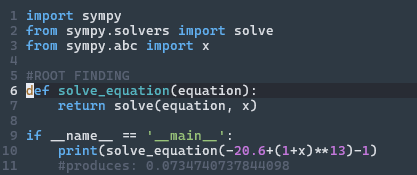
\includegraphics{./images/esungehw5q1.png}

\section{2.4.3}                                                                                                      
\begin{itemize}                                                                                                                              
	\item An annuity immediate has ten monthly payments of 1, and the quoted interest rate $i^{(4)}=8\%$. Determine its PV and its FV\\
        \item If the quoted rate is an annual effective rate of 6\%, find the PV and the fV of the annuity.                          
\end{itemize}
We are given quarterly interest so we have to make the necessary adjustments to get an annual representation. We then
use our equations for PV and FV to solve each of our stated problems.
\begin{itemize}
	\item $i$=8\%\\
\end{itemize}
$$
\begin{aligned}
	i^{(12)} &= m[\left(1+.06 \right)^{\frac{1}{m}} -1]\\
		 &= 12[\left(14.0824 \right)^{\frac{1}{12}} -1 ]\\
		 &= 7.94\%\\
	PV &= a_{\actuarialangle{10}7.94}\\
	   &= \frac{1-0.4655}{0.0744}\\
	   &= 6.73\\
	FV &= a_{\actuarialangle{10}7.94}\\
	   &= \frac{1-i^n}{i}\\
	   &= 14.45\\
\end{aligned}
$$

\begin{itemize}
	\item $i$=6\%\\
\end{itemize}
$$
\begin{aligned}
	i^{(12)} &= m[\left(1+.06 \right)^{\frac{1}{m}} -1]\\
		 &= 12[\left(14.0824 \right)^{\frac{1}{12}} -1 ]\\
		 &= 5.841\%\\
	PV &= a_{\actuarialangle{10}5.841}\\
	   &= \frac{1-0.548}{0.05841}\\
	   &= 7.48\\
	FV &= a_{\actuarialangle{10}5.841}\\
	   &= \frac{1-i^n}{i}\\
	   &= 13.08\\
\end{aligned}
$$

\section{2.5.2} 
A five year annuity has increasing monthly payment at the end of each month. The first payment
us 600, and each subsequent payment is 10 larger than the previous payment. At a rate of 
$0.5\%$ per month, find the PV of the annuity valued one month before the final payment.                                                                                                                                                                                  
Soln: There are at least two ways of approaching this problem. \\                                                                                                                                                                                                         

We can think of the 5 year annuity as a level annuity of [BLANK] per month,
and an increasing annuity annuity with additional payments of 10. We also
discount our additional payments.
$$                                                                                                                                   
\begin{aligned}
	PV &= 600a_{\actuarialangle{60}i} + 10 \left(Ia_{\actuarialangle{59}i}\right)v\\
	   &= 600a_{\actuarialangle{60}.005} + 10 \left(Ia_{\actuarialangle{59}.005}\right)v\\
	   &= 600(\frac{1-v^{20}}{i}) + 10 \left(\frac{a^{..}_{\actuarialangle{59}.005}-59v^{59}}{i}\right)v\\
	   &= 600 (51.7255) + 10(\frac{51.239-43.959}{0.005})v\\
	   &= 31,035.33+14,486.45\\
	   &= 45,521.79\\
\end{aligned}
$$                                                                                                                           
\pagebreak




\section{2.5.3}                                                                          
Jeff bought an increasing perpetuity-due (annuity due means its due at beginning of month
immediate is at the end of the month) with annual payments starting at 5 and increasing by 5
each year until the payment amount reaches 100. Thereafter, the payments then remain
at 100. If the annual effective rate is $7.5\%$, what is the PV of this perpetuity?\\

$Ia_{\infty}$ will be used (but at the period when this happens you need to discount it)
$$
Ia_{\actuarialangle{\infty}}v^{19}\\
$$
Starting from time 0 we will have a total of 20 payments (19 after our initial 5 at time zero) in order to reach 100. So our PV equation will
take the form of 2 terms accounting for the initial 5 and the increasing payments, and the final constant 
payments of 100 for an indefinite time (infinity).\\

$$
\begin{aligned}
	a_^{..}_{\actuarialangle{20}.075} &= \frac{1-v^{20}}{d} \\
					   &= 10.959\\
\end{aligned}
$$
$$
\begin{aligned}
	d &= \frac{i}{1+i}\\
	  &= 0.0697\\
\end{aligned}
$$
$$
\begin{aligned}
	PV &= 5Ia^{..}_{\actuarialangle{20}.075} + 100(a_{\actuarialangle{20}.075})v^{19}\\
	   &= 5(1.075)[\frac{a^{..}_{\actuarialangle{20}.075} -20v^{20}}{0.075}] + \frac{100}{0.075}v^{19}\\
	   &= 447.97 + 337.42\\
	   &= 785.40\\
\end{aligned}
$$
Hence, we find that the PV of the above perpetuity is $785.40$.


% --------------------------------------------------------------
%     You don't have to mess with anything below this line.
% --------------------------------------------------------------
 
\end{document}
